\noindent
The standard fitting model treats the sample as a \emph{thin} absorber:
the transmission is linear in the absorption of each component. In thick
or strongly absorbing samples this approximation fails —the deep lines \emph{saturate}—
and it biases depths, widths and, above all, the areas (phase fractions).
The experimental branch adds a \emph{thickness correction} through a
saturation model with a single physical parameter $C$. This document explains
what benefits it brings, when it is worth applying, how it is applied (what
changes in the fit and in the display) and how it behaves with several subspectra.



\bigskip

%======================================================================
\section{The problem: thin vs. thick absorber}

The historical model is linear in the absorption:
\begin{equation}
  T_{\text{delgado}}(v) \;=\; b + s\,v \;-\; A_{\text{tot}}(v),
  \qquad A_{\text{tot}}(v)=\sum_{c} A_c(v),
  \label{eq:thin}
\end{equation}
with $b$ the baseline, $s$ the slope and $A_c$ the absorption of each component
(sextet/doublet/singlet). It is exact only in the limit of an
infinitely thin absorber. In a real sample of finite thickness, the fraction of
resonant photons that reach the detector decays \emph{exponentially} with the amount of
resonant material: the deepest lines absorb proportionally less than
\eqref{eq:thin} predicts (they \emph{saturate}) and, in addition, they \emph{broaden}.

\begin{nota}
The thickness saturation effect is not a numerical artifact: it is physics of the
transmission experiment. Ignoring it in thick samples makes the fit falsely
``compensate'' by raising widths and unbalancing areas.
\end{nota}

%======================================================================
\section{Exponential saturation model}

The correction replaces \eqref{eq:thin} with
\begin{equation}
  \boxed{\;
  T(v) \;=\; b + s\,v \;-\; C\,\Bigl(1 - e^{-A_{\text{tot}}(v)/C}\Bigr)
  \;}
  \label{eq:thick}
\end{equation}
where $C>0$ is the \emph{saturation scale} (the maximum achievable absorption
amplitude, $\approx f_s\,b$, with $f_s$ the effective recoil-free fraction
of the source). Its two limits make it interpretable and backward compatible:
\begin{itemize}[leftmargin=*]
  \item \textbf{Thin limit} $C\to\infty$: since $C(1-e^{-x/C})\to x$, one
        recovers \eqref{eq:thin} exactly. That is, the thin model is the
        particular case of zero thickness.
  \item \textbf{Saturation} $C$ finite: the effective absorption
        $A_{\text{eff}}=C(1-e^{-A_{\text{tot}}/C})$ is bounded by $C$ and
        compresses the deep lines the more, the larger
        $A_{\text{tot}}/C$ is.
\end{itemize}
Implemented in \code{core/physics.py} (\code{total\_model}, parameter
\code{sat\_scale}=$C$).

\begin{figure}[htbp]\centering
  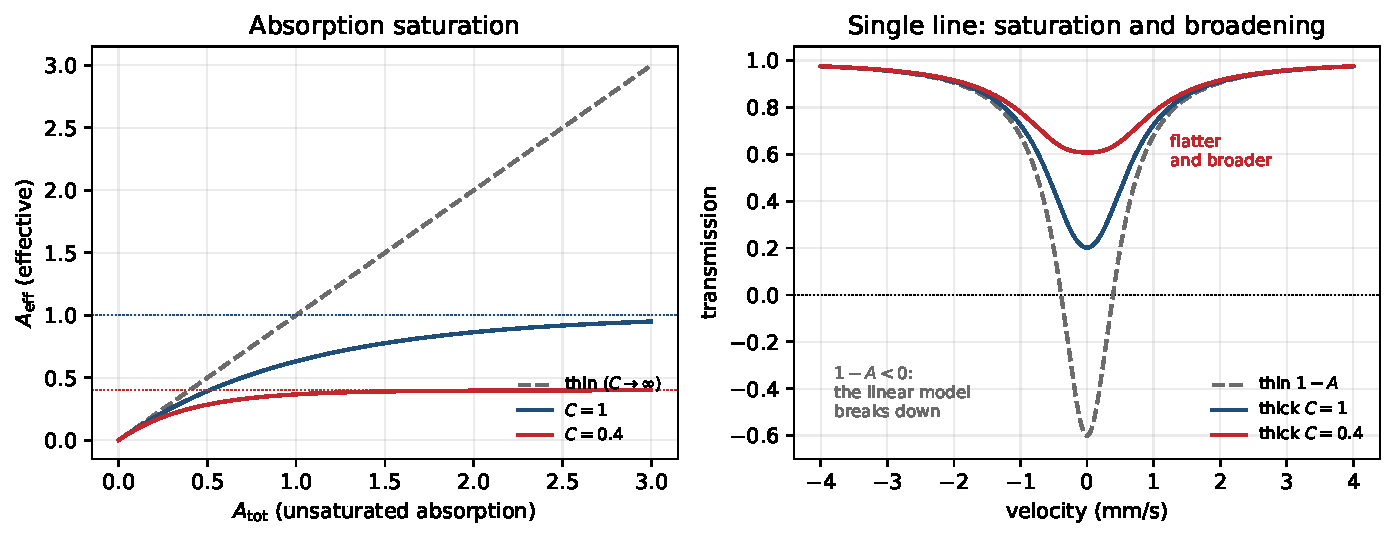
\includegraphics[width=0.98\textwidth]{apx_thickness}
  \caption{Thin versus thick absorber. \emph{Left}: the effective
  absorption $A_{\text{eff}}=C(1-e^{-A_{\text{tot}}/C})$ saturates, bounded by $C$,
  while the thin model ($C\to\infty$) grows without limit. \emph{Right}:
  over a deep line, the thin model $1-A$ would reach impossible negative
  values; the thickness correction gives \emph{shallower and broader}
  lines, which is the physical effect of saturation.}
  \label{fig:apx_thickness}
\end{figure}

%======================================================================
\section{Benefits}

\begin{enumerate}[leftmargin=*]
  \item \textbf{Unbiased areas and phase fractions.} Saturation suppresses
        the absorption of the majority phases (deep lines) more than that of the
        minority ones. Without correction, the area ratio is biased in favor of
        the weak phases. By \emph{de-saturating}, the recovered areas
        correspond to those of the equivalent thin absorber, which are the ones
        proportional to the abundances (at equal Lamb–Mössbauer $f$).
  \item \textbf{Correct depths.} The depth parameter no longer reads
        the apparent (clipped) absorption but represents the real absorption.
  \item \textbf{Less inflated widths.} The thickness broadening is no longer
        artificially absorbed into $\gamma$; the fitted widths approach the
        intrinsic ones.
  \item \textbf{Better $\chi^2$ in deep spectra.} Where the thin model
        leaves systematic structure in the residual (at the minima), saturation
        removes it without adding spurious components.
\end{enumerate}

\begin{nota}[Verification]
On a synthetic spectrum saturated with $A_{\max}/C=2$, the fit with thickness
correction reconstructed the spectrum $\sim27\%$ better (RMS) than the thin
model, and recovered the starting scale $C$ ($C=0.41$ versus the true
$0.40$). In mild saturation it recovered $\sim9\%$ more area (de-saturation).
\end{nota}

%======================================================================
\section{When to apply it}

\begin{aviso}
The thickness correction \textbf{helps} when the sample is thick / strongly
absorbing and \textbf{is not necessary} (and should not be forced) when it is thin.
\end{aviso}

Signs that it is worth enabling it:
\begin{itemize}[leftmargin=*]
  \item Deep absorption: the transmission minimum drops well below the
        baseline (typically $\gtrsim 15$–$20\%$ absorption), or effective thickness
        $t_a\gtrsim 1$.
  \item The thin fit leaves \emph{structured residual at the minima} (the
        model does not reach the bottom of the deep lines or makes them too
        wide).
  \item Reliable \emph{phase quantification} is sought (area ratios), not
        just positions.
\end{itemize}
When \emph{not}:
\begin{itemize}[leftmargin=*]
  \item Thin spectra (absorption of a few \%): the linear model is already exact and
        $C$ is undetermined (it tends to large values). Keep thin mode.
  \item As a diagnostic: if, when $C$ is fitted, it converges to a large value and
        the $\chi^2$ does not improve, the sample is effectively thin.
\end{itemize}

%======================================================================
\section{How it is applied in the fit}

\subsection{Selection and parameter}
In the \emph{Velocity, folding and background} panel there is an \emph{Absorber}
selector with three options: \emph{Thin (linear)} (\code{thin}), \emph{Thick
(saturation)} (\code{thickness}) and \emph{Transmission integral}
(\code{transmission}). In thick mode the saturation-scale $C$ \emph{slider}
(\code{sat\_scale}) appears. $C$ is a global parameter
(like the baseline or the slope), adjustable or fixable.

\subsection{Discrete mode}
The nonlinear optimizer (TRF) already fits an arbitrary function, so it is enough
for the forward model to use \eqref{eq:thick}: $C$ enters as one more free
parameter and is refined together with the rest. The algorithm does not change,
only the forward model.

\subsection{Distribution mode: not applied}
The distribution fit always assumes a \textbf{thin} absorber: the thickness
correction is \emph{not implemented} in distribution mode, whatever the selector
says. The reason is that the exponential \emph{breaks the linearity} in the weights
$P$, on which the whole regularized solver relies (non-negativity, $\alpha$,
$1\sigma$ band, L-curve). The distribution panel shows a warning when the selector
is not on \emph{Thin}.

In a thick sample, a distribution fitted as thin absorbs the thickness effect: it
comes out somewhat broader, with relative areas biased towards the weak lines.
Thin samples are advisable for distributions; when that is not possible, a
discrete fit in thick mode, compared with the thin one, shows how much widths
and areas change.

%======================================================================
\section{What changes in the view}

\begin{itemize}[leftmargin=*]
  \item The displayed \textbf{model curve} is the \emph{saturated} transmission
        \eqref{eq:thick}: it is the one compared with the data and the one that
        generates the residual.
  \item The displayed and exported \textbf{depths/areas} are those of the
        equivalent thin absorber (de-saturated): for this reason, when the
        correction is enabled, the relative areas may change with respect to the thin
        fit —which is precisely the intended correction.
  \item The fitted value of $C$ (saturation scale) appears among the
        global parameters. A large $C$ indicates a practically thin sample.
\end{itemize}

%======================================================================
\section{Several subspectra}

Saturation is a property of the \emph{whole absorber}, not of each phase
separately: the photons of a given velocity pass through all the material and
``see'' the sum of all the absorptions at that velocity. That is why \eqref{eq:thick}
saturates the \textbf{total absorption} $A_{\text{tot}}=\sum_c A_c$ with a
\emph{single} scale $C$ common to all subspectra, and not each component
on its own:
\begin{equation}
  T(v) = b + s\,v - C\Bigl(1 - \exp\!\bigl[-\tfrac{1}{C}\textstyle\sum_c A_c(v)\bigr]\Bigr).
\end{equation}
Practical consequences:
\begin{itemize}[leftmargin=*]
  \item \textbf{Correct physical coupling.} Where two subspectra overlap, the
        saturation is larger (the local absorption is the sum); the model captures it
        automatically.
  \item \textbf{Phase quantification.} After de-saturating, the area ratios
        between subspectra recover their unbiased value, which is the goal in
        phase mixtures (e.g. several Fe environments).
  \item \textbf{A single $C$.} A scale per component is not fitted (it would be
        unphysical and would degenerate with the depths): $C$ is global and describes the
        effective thickness of the sample.
\end{itemize}

\begin{nota}[Model limitation]
It is an effective exponential saturation (Lambert–Beer), which captures the
dominant thickness effect (compression, broadening, unbiased areas) with a single
parameter. For the full treatment, the \emph{Transmission integral} option
convolves the source line with $1-e^{-\tau(v)}$, as NORMOS does, with the source
width and its resonant fraction as global parameters.
\end{nota}

%======================================================================
\section{Summary}

\begin{center}
\begin{tabular}{@{}ll@{}}
\toprule
\textbf{Aspect} & \textbf{Thickness correction}\\
\midrule
Model & $T=b+s v - C(1-e^{-A_{\text{tot}}/C})$ \\
New parameter & $C$ (saturation scale), global, $C\to\infty$ = thin\\
When & thick samples / deep absorption / phase quantification\\
Discrete & $C$ free in the TRF; only the forward model changes\\
Distribution & not applied: a thin absorber is assumed (the panel warns)\\
View & saturated curve; areas de-saturated; $C$ is shown\\
Subspectra & a single $C$ saturates the sum $\sum_c A_c$ (physical coupling)\\
Key benefit & unbiased areas/phase fractions, better widths and $\chi^2$\\
\bottomrule
\end{tabular}
\end{center}
